% Chapter 2 of the Thesis Template File
%   which includes bibliographic references.

%Chapter 2 goes over the theory of operation for a radiometer and specifically the theory of operation of how a traditional radiometer is carried over to one using a SDR.  General information of the N200 and GNURadio and why they were picked for this project is also discussed.  This chapter will introduce the reader to overall solution to the problem and their use for the new radiometer system to be used.

\chapter{THEORY OF OPERATION}

The work of this thesis is to use a software defined radio (SDR) to replace the bulk of the digital components used on the ISU radiometer.  In many ways, the existing ISU radiometer is very much like a SDR in that it employed an A/D converter and FPGA to process the signal.  However, these devices were designed specifically to look at the overall power of the incoming signal.  It was desired that we have the capability to look at the full signal coming so that a more in depth analysis can be performed.  For this reason, a new approach is devised to use off the shelf hardware and the logical choice was an off the shelf SDRs which can offer similar performance while expanding on the functionality of the radiometer.  The advantages of being able to look at the whole signal instead of just power will be discussed later in this thesis.

The hardware that was selected for this research was the Ettus Research N200 Software Defined radio.  Information and rationale behind the selection of this unit will be covered later.  The N200 however gives us the standard building blocks for a typical software defined radio which includes a A/D converter and on-board FPGA.  The N200 however also gives a flexible front end by selecting various daughter boards that fit our application.  In addition, the N200 supports up to two daughter boards to be installed.  

A software defined radio of course is only as good as the software that is written to work with the hardware.  As the name implies, the software defines how the radio will act and function.  From a computer engineering perspective though, software can take on several roles in a system.  There is software that runs on the hardware, in our case the FPGA, and then there is software that may run on a computer to interface with the hardware.  In some cases, the software may only reside on the hardware, however, to increase the user usability of the system, we will be using a combination of firmware that is running on the FPGA and software that runs on a computer.  GNURadio is an open source software define radio framework that runs on multiple OSes and offers a rich set of features.  In addition, GNURadio is well supported by the Ettus Research group and is the preferred software for interfacing with their hardware.  An easy to use interface was another driving requirement for our implementation of a radiometer in a SDR.  GNURadio helps us with this through the use of the GNU Radio Companion or GRC.  This was important as it was anticipated that many operators of the radiometer would not know much about programming.  GNURadio uses a simple to use graphical system that is very similar to things such as LabView, offering a drag and drop system for adding various radio components such as filters.  Like LabView, you can also simply wire up the boxes and complete the circuit path for the RF signal as it gets processed.

\section{Radiometer Theory of Operation}

The primary goal of a radiometer is to measure power.  While that statement sounds easy, there are in fact many factors that go in to how well a radiometer can measure the power it sees.  A better statement would be that a radiometer's primary goal is to accurately measure power within a certain degree of accuracy.  In order to accurately and within a high degree of precision measure power, a radiometer must take into account various factors such as the system noise, the bandwidth of the signal and the stability of the system as a whole.  

\subsection{Measuring RF power}

To measure power in a radiometer, several factors are taken into consideration.  To begin with we have the noise signal coming from the antenna.  Our antenna is assumed to be looking at our target of interest and it is assumed that we can relate the antenna noise to the noise from the source.  It is often easier to refer to this noise as the brightness temperature.  Therefore the brightness temperature of the source can be related to the brightness temperature at the antenna.  We will refer to this brightness temperature as T$_{A}$.  

{\begin{figure}[h!tb] 
\centering
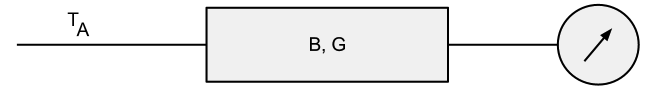
\includegraphics[width=\textwidth]{Images/simple_rad.png}
\isucaption{The ideal radiometer block diagram}
\label{simplerad}
\end{figure}
}

Figure~\ref{simplerad} shows us an ideal radiometer.  That is a radiometer that has an input from the antenna, T$_{A}$, a known bandwidth denoted as B and a known gain denoted as G.  At the end of the block is the detector, which measures the power from the radiometer.

Only a certain selection of the radio spectrum is observed by the radiometer.  This is referred to as the bandwidth of the radiometer and is denoted as B or as $\beta$.  This bandwidth is then centered around a center frequency.  In our case, we center around 1.405 GHz.  There is a reason why 1.405 GHz is selected.  The range from 1.4 to 1.426 MHz is protected internationally.  This reduces interference from outside sources such as transmitters that can interfere with the operation of the radiometer.  

The power coming from the antenna is amplified so it is easier to determine changes in the brightness temperature.  The overall gain of the radiometer system is referred to as G in this case.  Finally, we need to apply Boltzmann's constant, referred to as \textit{k}.  With these values, we can now compute the power the radiometer will see for an ideal radiometer.  This can be shown in equation~\ref{eq:power_rad_eq}

\begin{equation} \label{eq:power_rad_eq}
P=k*\beta*G*(T_{A})
\end{equation}

However, since we do not have an ideal radiometer, we have another key component that needs to be addressed.  This is the noise that is added to the system by the radiometer itself, primarily from the amplifiers used to increase the signal.  Most of the additional noise is from the Low Noise Amplifiers (LNA) that are used to increase the signal while attempting to keep the noise added to a minimum.  However, noise is also added from virtually every component in the RF front end.  However, by far the largest contribution usually comes from the LNA, which is why the selection of the LNAs is a critical decision.  Figure~\ref{noiserad} shows the additional noise that is injected into the system.

{\begin{figure}[h!tb] 
\centering
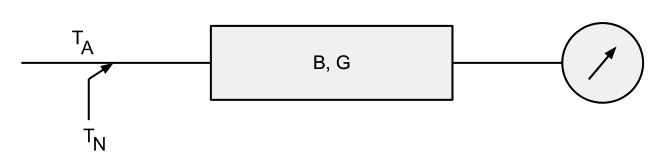
\includegraphics[width=\textwidth]{Images/radiometer_noise_added.png}
\isucaption{A more realistic radiometer model}
\label{noiserad}
\end{figure}
}

As it can be seen, this additional noise is added to the noise coming from the antenna source.  Therefore T$_{N}$ is added to T$_{A}$ and our final equation for the power measured is shown in equation~\ref{eq:final_power}.  

\begin{equation} \label{eq:final_power}
P=k*\beta*G*(T_{A}+T_{N})
\end{equation}

The issue with all radiometers is that it must detect small signal changes in a noisy environment.  To understand this, let us look at the example of T$_{A}$ has a value of 200 K and T$_{N}$ has a value of 800 K.  Since T$_{N}$ is added to our antenna signal, we have a total noise temperature of 1,000 K.  This means that if we want to detect a change as small as 1 K, we must be able to measure the difference between 1,000 K and 1,001 K. [\cite{skou}]

The ability of a radiometer to detect these small changes is the radiometer's sensitivity, or the standard deviation of the output signal from the radiometer.  This sensitivity is also referred to as the Noise Equivalent $\Delta$ Temperature or NE$\Delta$T. 

\begin{equation}
NE\Delta T=\frac{T_{A}+T_{N}}{\sqrt{\beta + \tau}}
\end{equation}

The sensitivity of the radiometer is based on both the bandwidth, $\beta$, of the incoming signal and the integration time, $\tau$.  As it can be seen in the equation, we would want to have as much bandwidth as possible.  In a traditional radiometer, this bandwidth is often fixed and is dependent on the band-pass filters used in the radiometer.  We can however control $\tau$ and a longer integration time will help improve the sensitivity of the radiometer.[\cite{skou}]

This covers a very simplified radiometer, however most radiometers are more complicated than the one shown in Figure~\ref{noiserad}.

%Insert a graph like the one found in Skou, Figure 4.1

A more typical radiometer can be shown in Figure .  Here we have expanded the blocks used and have separated the bandwidth and gain blocks.  In addition, we have detection, shown as X$^2$, and integration.  These last two blocks make up the detection and results in the power we can measure, which is a voltage represented as V$_{out}$.  This results in equation~\ref{eq:vout_1}.

\begin{equation} \label{eq:vout_1}
V_{OUT}=c*(T_A+T_N)*G
\end{equation}

Here V$_{OUT}$ is shown by the addition of both the noise from the system T$_N$ and the noise from the antenna, T$_A$ and multiplied by the gain in the system, G.


\section{Software Defined Radio Theory of Operation}

A software defined radio (SDR) attempts to mimic radio functions in software instead of relying on dedicated hardware.  As stated in the previous section, a radiometer is a radio that can detect changes in power.  Therefore the SDR needs to be able to measure power coming from the source that we are looking at.  

The SDR is able to do all of this but in a slightly different way than a traditional radiometer.  A traditional radiometer will use a device called a square-law detector to measure the incoming RF signal.  This device is simply a diode where the input voltage is squared and the output from the diode is proportional to the AC input voltage.  Therefore a 3 dB increase in the RF power will result in a two times increase in the voltage.  This power measurement will be fluctuating rapidly, therefore we will then run the output from the square-law detector to an integrator and integrate over a set time period.  As shown in equation 2.5, this integration time also affects the NE$\Delta$T or sensitivity of the radiometer as well.

For the SDR, the incoming signal is sampled and converted to IQ values.  The IQ values represent the amplitude and phase information of the signal.  In GNURadio we are then able to square these values within software.  This block in GNURadio mathematically performs the following:

\begin{equation}
I^2+Q^2 = P_{out}
\end{equation}

Like the analog square-law detector, this signal will fluctuate rapidly and to improve the sensitivity of the radiometer we wish to integrate this signal.  A RC filter is analogous to an integrator where the R and C values determine our time constant and our integration time for the filter.  A SDR however operates in the digital domain at discrete intervals.  One type of filter that can be used in the Infinite Impulse Response (IIR) filter. 

To begin with, we look at what an analog RC filter looks like. 

{\begin{figure}[h!tb] 
\centering
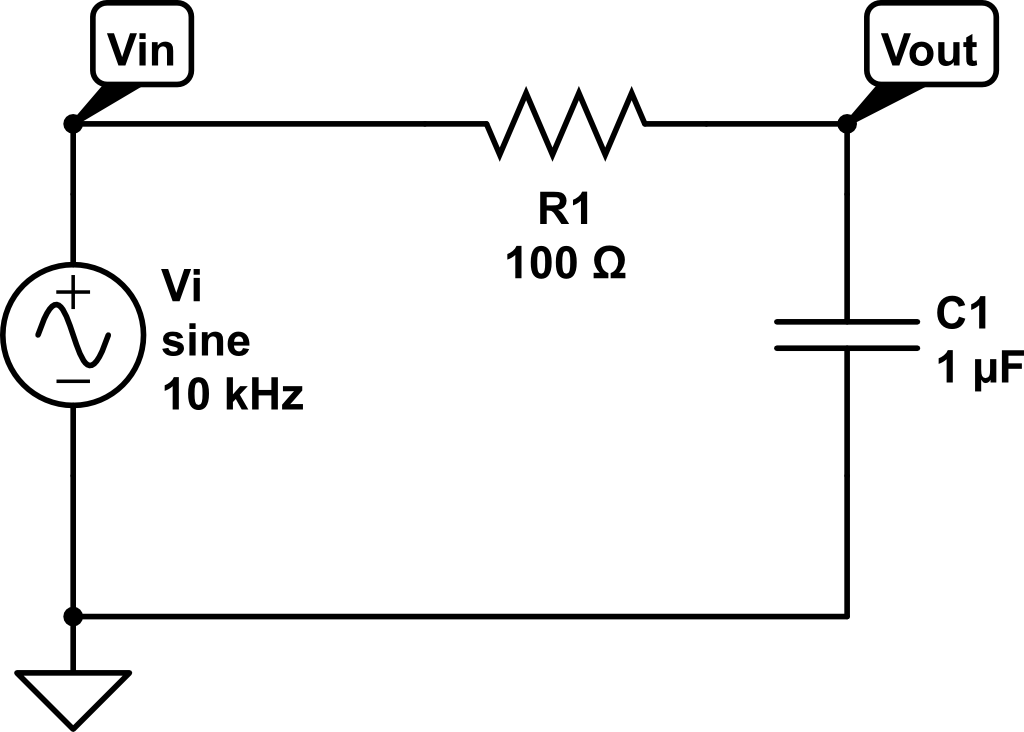
\includegraphics[width=\textwidth]{Images/rc-circuit.png}
\isucaption{A simple RC circuit}
\label{rc_circuit}
\end{figure}
}

This circuit can be represented by the following equation.
\begin{equation}
\frac{V_{in}-V_{out}}{R}=C\frac{dV_{out}}{dt}
\end{equation}

A Finite Impulse Response (FIR) filter is a digital filter that can take an impulse signal and decays to zero after a finite number of iterations.  This type of digital filter can be represented by the following equation:

\begin{equation}
y_n=\displaystyle\sum\limits_{i=o}^{P-1} c_ix_{n-i}
\end{equation}

This simply says that the nth output is a weighted average of the most recent P inputs.  

An Infinite Impulse Response (IIR) filter is the same as the FIR filter, except that we add an additional summation term which feeds back the previous output.

\begin{equation}
y_n=\displaystyle\sum\limits_{i=o}^{P-1} c_ix_{n-i}+\displaystyle\sum\limits_{j=1}^{Q} d_jy_{n-j}
\end{equation}

It can be seen that a FIR filter is really a IIR filter except that $Q=0$.  

To get a better understanding on how our digital IIR filter relates to our RC filter analog, we can look at the Fourier Transform and the relationship of the input to the output in the frequency domain.

\begin{equation}
H(f)=\frac{\displaystyle\sum\limits_{j=o}^{P-1} c_je^{-2\pi ijfT}}{1-\displaystyle\sum\limits_{k=1}^{Q} d_ke^{-2\pi ikfT}}
\end{equation}

Here $f$ is our frequency in Hz and $T$ is the time between samples in seconds.

We now want show the link between our analog RC circuit and the IIR filter.  Looking at equation 2.6, which represents the differential equation relating the input voltage $V_{in}$ to the output voltage $V_{out}$, we can subsitute for input and output of our IIR filter.  Since we are now in the time domain, we need to define what $T$ is.

\begin{equation}
T=time between samples=\frac{1}{sampling rate}
\end{equation}

We can now relate our input voltage to the input to our IIR filter and the output voltage to the output of our IIR filter.

\begin{equation}
x_n=v_{in}(nT)
\end{equation}

\begin{equation}
y_n=v_{out}(nT)
\end{equation}

We can now rewrite our difference equation with $x_n$ and $y_n$.

\begin{equation}
\frac{x_n-y_n}{R}=C\frac{y_n-y_{n-1}}{T}
\end{equation}

Now, we can solve for $y_n$ which results in our final equation for showing how a IIR filter is related to an RC filter.

\begin{equation}
y_n=\frac{T}{T+RC}x_n+\frac{RC}{T+RC}y_{n-1}
\end{equation}

It can be seen that an IIR filter can have the same frequency response as we would expect from an analog RC filter.  As our sampling rate approaches infinity, the approximation gets closer to the original response from the analog RC circuit.  

For the cutoff frequency of a RC circuit, we know that it has the following relationship.

\begin{equation}
f_c=\frac{\sqrt{3}}{2\pi RC}\rightarrow RC=\frac{\sqrt{3}}{2\pi f_c}
\end{equation}

The $RC$ term gives us our time constant of the circuit and can be used to calculate out our coefficients.  We are not concerned about the actual values of R and C with our IIR filter, instead we just need the product of R and C.  

For GNURadio most of the work is done for us.  We can simply enter in our desired cutoff frequency and GNURadio will calculate our IIR filter coefficients.  However, this shows that an IIR filter works very much like an analog RC low pass filter.

Like a traditional radiometer, the SDR will use an antenna to look at the target of interest.  SDRs still use a RF stage that takes the power from the source and amplifies it.  The difference though begins after that.  A SDR will then sample and generate I and Q values that represents the amplitude and phase of the signal.  From there, this data is sent to a computer to be processed.  We can then use this information to calculate the power that is being seen.  In addition, we can manipulate the signal in other ways such as applying a filter to filter out an unwanted source.


The N200 is a SDR developed and built by Ettus Research.  It is one of the newer models in the companies USRP line of SDRs.  It offers several key features that were desirable for a radiometer type of application while still being an economical option.  It also offered a highly flexible architecture which will allow this radio to be up-gradable in the foreseeable future.  

{\begin{figure}[h!tb] 
\centering
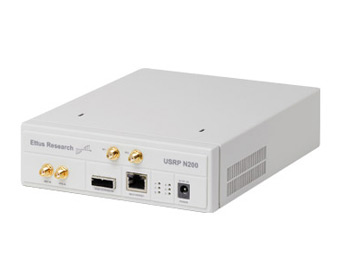
\includegraphics{Images/n200}
\isucaption{The USRP N200 from Ettus Research}
\label{N200}
\end{figure}
}
\subsection{General Specifications}

The N200 has the following features that made it well suited for our specific application.

\begin{itemize}
\item Dual 14-bit ADC
\item Dual 16-bit DAC
\item 50 MS/s Gigabit Ethernet streaming
\item Modular daughter-board system for RF front end
\end{itemize}

These specifications had a large impact on the selection of the N200 for this application.  Specifically the 14-bit ADC, the 50 MS/s and the modular daughter-board system were the largest factors in the decision to use the N200 SDR.  Further explanation on these specifications are explained in the following sections.

\subsubsection{14-bit ADC}
The analog to digital converters (ADC) allow us to take the analog I and Q values from the daughter boards and digitize this information.  Once digitized, we can now work with the signal both on the on-board FPGA board or stream it to the computer so that our software can manipulate the signal.  In radiometry, we are primarily looking at the overall power of the signal and this does not require us to accurately recreate the signal.  However, it will be discussed in this paper in further detail that there are times where being able to recreate the signal for additional analysis can be quite beneficial.  For that reason, the resolution of the ADC becomes more important.

% Below \subsubsection
% Sectional commands: \paragraph and \subparagraph may also be used
\subsubsection{50 MS/s Bandwidth}
For this application, the N200 is required to receive a signal at 1.4 GHz and is at least 20 MHz wide.  Bandwidth plays an important role in remote sensing and to the amount of power that we receive.  It also plays a key role in the sensitivity of the radiometer.  To begin, an examination of how much power that is received and the correlation to the bandwidth will be looked at.

\begin{equation}
P=k*\beta*G*(T_{A}+T_{sys})
\end{equation}

Here we can see that the bandwidth of the signal received directly relates to the amount of power the radiometer will measure.  The higher the bandwidth the more power the radiometer will see.  

Equally important however is the the sensitivity or how small of a change the radiometer can detect.  This sensitivity or NEAT function is shown in equation 2.2

\begin{equation}
NE\Delta T=\frac{T_{A}+T_{sys}}{\sqrt{\beta + \tau}}
\end{equation}

Again, the amount of bandwidth the radiometer receives plays a large part in the performance of the radiometer.  

Another factor however is the amount of bandwidth the existing RF front end of the ISU radiometer is able to provide to us.  The current filters on the ISU Radiometer keep the bandwidth of the signal to 20 MHz.  This meant that at the very minimum a 20 MS/s bandwidth from the SDR is required.  

The N200 is capable of working with up to 100 MS/s signal and can stream up to 50 MS/s through the Gigabit Ethernet connection.  The N200 also has the ability to have up to 2 daughter boards installed.  If we assume each will have up to a 20 MHz signal, this means up to 40 MS/s of data will be required.  This means that the N200 meets are minimum requirements for working with needed bandwidth of the radiometer.  In addition, the FPGA on the N200 is capable of working with up to 100 MS/s, so there is room handling additional bandwidth by using the on board FPGA to process the signal.

\subsubsection{Daughter Boards}

The daughter boards allow for easy replacement of the RF front end to the software defined radio.  Ettus Research makes a number of daughter boards that range from a a wide range of frequencies and is available with transmitters, receivers and transceivers.  Because these boards are modular and do not touch the analog to digital converters or the on-board FPGA, very little change is required in the software.  The daughter boards however do have the required RF hardware for the signal to be processed.  In this application it was required that the signal was detected at 1.4 GHz with a bandwidth of 20 MHz.  The DBSRX2 receiver met this requirement and was selected to be used with the N200.  In this radiometer application transmission is not needed and is in fact illegal in the 1.4 GHz band, which is reserved for radiometer applications.

%\subsubsection{Parts of the second hypothesis}

%Here one particular part of the hypothesis that is 
%currently being explained is examined and particular
%elements of that part are given careful scrutiny.

\subsection{The DBSRX2 Receiver}
The DBSRX2 receiver board is capable of receiving signals between 800 MHz and 2.3 GHz.  The board is able to plug into one of expansion slots available on the N200 that we are using.  

The DBSRX2 has an onboard Programmable Gain Amplifier (PGA) that is accessible from the software and allows us to control the gain through GNURadio.  

{\begin{figure}[h!tb] 
\centering
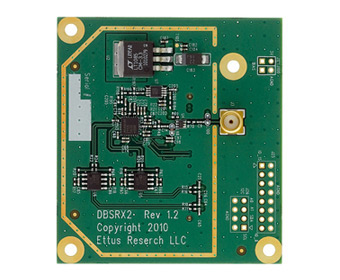
\includegraphics{Images/dbsrx2}
\isucaption{The DBSRX2 daughter board from Ettus Research}
\label{mgraph}
\end{figure}
}

\section{GNURadio}

GNURadio fills in the software side of the software defined radio.  Although there is firmware that runs on the FPGA in the N200, this firmware is designed to communicate with a host PC.  It is this software that does most of the work in terms of the calculations that are done with the signal.  The FPGA simply sends the raw IQ data to the host PC, which then performs the necessary math functions.  Again, the reason why software defined radios are desirable is the ability to change the behavior of the radio very quickly.  In our case we can change functionality by simply loading a new software program in the host PC.  

This functionality is ideal for communication type of radios where different modulation schemes and encoding and decoding methods can easily be changed out.  However, in a radiometer we are not interested in this aspect of the SDR.  However, one functionality is available that can be very valuable for a radiometer, and that is with filtering.  Although we often use frequencies that should be free from interference, this is not always the case.  Interference can and often does still occur, even in these protected frequencies.  With the SDR, we are able to quickly adapt to changing conditions by moving the frequency, changing our bandwidth and even filter out an offending signal.  

GNURadio was selected as it is an open source software platform.  GNURadio is licensed under the GPL license and has a strong community that continually updates the software.  It is also well supported by third parties such as Ettus Research Group, National Instruments and other SDR developers.  In addition GNURadio has a strong set of tools that can be used to develop programs that run under GNURadio.  Tools such as the GNURadio Companion (GRC) allows for an easy to use GUI to develop code for GNURadio.  GNURadio is also written in Python, which allows for easy modification and access to additional tools that can be used with GNURadio.  



